\documentclass[10pt]{beamer}\usepackage[]{graphicx}\usepackage[]{color}
%% maxwidth is the original width if it is less than linewidth
%% otherwise use linewidth (to make sure the graphics do not exceed the margin)
\makeatletter
\def\maxwidth{ %
  \ifdim\Gin@nat@width>\linewidth
    \linewidth
  \else
    \Gin@nat@width
  \fi
}
\makeatother

\definecolor{fgcolor}{rgb}{0.345, 0.345, 0.345}
\newcommand{\hlnum}[1]{\textcolor[rgb]{0.686,0.059,0.569}{#1}}%
\newcommand{\hlstr}[1]{\textcolor[rgb]{0.192,0.494,0.8}{#1}}%
\newcommand{\hlcom}[1]{\textcolor[rgb]{0.678,0.584,0.686}{\textit{#1}}}%
\newcommand{\hlopt}[1]{\textcolor[rgb]{0,0,0}{#1}}%
\newcommand{\hlstd}[1]{\textcolor[rgb]{0.345,0.345,0.345}{#1}}%
\newcommand{\hlkwa}[1]{\textcolor[rgb]{0.161,0.373,0.58}{\textbf{#1}}}%
\newcommand{\hlkwb}[1]{\textcolor[rgb]{0.69,0.353,0.396}{#1}}%
\newcommand{\hlkwc}[1]{\textcolor[rgb]{0.333,0.667,0.333}{#1}}%
\newcommand{\hlkwd}[1]{\textcolor[rgb]{0.737,0.353,0.396}{\textbf{#1}}}%
\let\hlipl\hlkwb

\usepackage{framed}
\makeatletter
\newenvironment{kframe}{%
 \def\at@end@of@kframe{}%
 \ifinner\ifhmode%
  \def\at@end@of@kframe{\end{minipage}}%
  \begin{minipage}{\columnwidth}%
 \fi\fi%
 \def\FrameCommand##1{\hskip\@totalleftmargin \hskip-\fboxsep
 \colorbox{shadecolor}{##1}\hskip-\fboxsep
     % There is no \\@totalrightmargin, so:
     \hskip-\linewidth \hskip-\@totalleftmargin \hskip\columnwidth}%
 \MakeFramed {\advance\hsize-\width
   \@totalleftmargin\z@ \linewidth\hsize
   \@setminipage}}%
 {\par\unskip\endMakeFramed%
 \at@end@of@kframe}
\makeatother

\definecolor{shadecolor}{rgb}{.97, .97, .97}
\definecolor{messagecolor}{rgb}{0, 0, 0}
\definecolor{warningcolor}{rgb}{1, 0, 1}
\definecolor{errorcolor}{rgb}{1, 0, 0}
\newenvironment{knitrout}{}{} % an empty environment to be redefined in TeX

\usepackage{alltt}%
\usetheme{Boadilla}
\usecolortheme{seahorse}

\usepackage[utf8]{inputenc}%


\usepackage[normalem]{ulem}%strikeout
 

% graphics
%% Figures %%%%%%%%%%%%%%%%%%%%%%%%%%%%%%%%%%%%%%%%%%%%%%%%%%
\usepackage{graphicx}
\usepackage{xcolor}%for color mixing

\usepackage{amsmath}%
\usepackage{amsfonts}%
\usepackage{amssymb}%
\usepackage{graphicx}

\usepackage{tikz}
\usetikzlibrary{calc}

%%%%%%%%%%%%%%%%%%%%%%%%%%%%%%%%%%%%%%%%%%%%%%
%%%%%%%%%%%%%%%%% Doc info %%%%%%%%%%%%%%%%%%%
\title[\textbf{Generalized linear models:}]{Generalized Linear Models (GLMs)}
\date{\today}

%%%%%%%%%%%%%%%%%%%%%%%%%%%%%%%%%%%%
\IfFileExists{upquote.sty}{\usepackage{upquote}}{}
\begin{document}




\begin{frame}
\maketitle
\end{frame}
%%%%%%%%%%%

\AtBeginSection[]
{
  \begin{frame}<beamer>
    \frametitle{}
    \tableofcontents[currentsection,hideothersubsections,subsectionstyle=hide]% down vote\tableofcontents[currentsection,currentsubsection,hideothersubsections,sectionstyle=show/hide,subsectionstyle=show/shaded/hide]
  \end{frame}
}



%%%%%%%%%%%%%%%%%%%%%%%%%%%%%%%%%%%%%%%%%%%%%%%%%%%%%%%%%%%%%%%%%%%
%%%%%%%%%%%%%%%%%%%%%%%%%%%%%%%%%%%%%%%%%%%%%%%%%%%%%%%%%%%%%%%%%%%
\section{Linear model, reminder}

\begin{frame}[fragile]{A simple linear model}
  \textbf{{\color{purple}{Response}} = {\color{blue}{Intercept}} + {\color{red}{Slope}} $\times$ {\color{orange}{Predictor}} + {\color{gray}{Error}}} \\

\begin{knitrout}\small
\definecolor{shadecolor}{rgb}{0.843, 0.867, 0.922}\color{fgcolor}
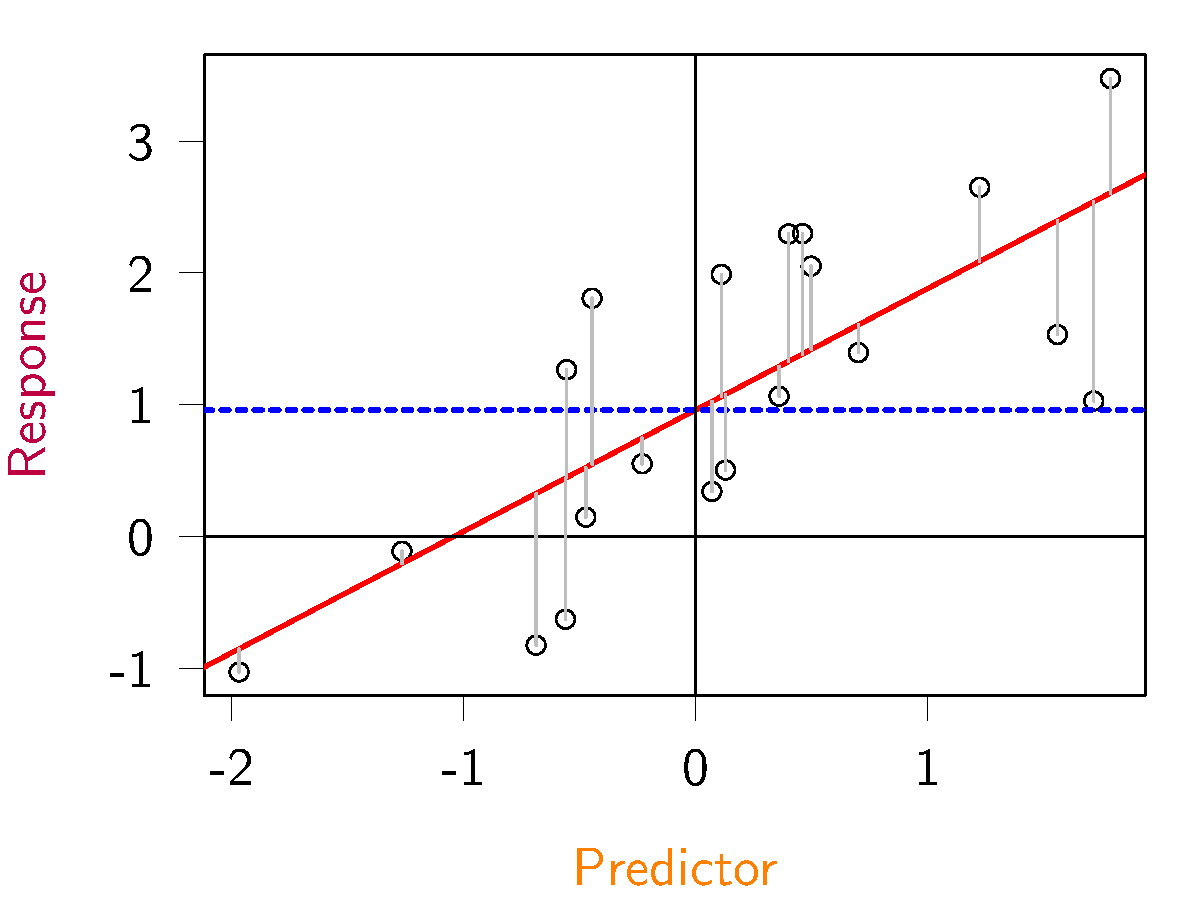
\includegraphics[width=0.8\textwidth,height=0.6\textwidth]{figure/lmprinc-1} 

\end{knitrout}
\end{frame}
%%%%%%%%%%%

\begin{frame}[fragile]{A simple linear model failure: binary data}

\begin{knitrout}\small
\definecolor{shadecolor}{rgb}{0.843, 0.867, 0.922}\color{fgcolor}
\includegraphics[width=0.8\textwidth,height=0.6\textwidth]{figure/binlmprinc-1} 

\end{knitrout}
  
\end{frame}
%%%%%%%%%%%

\begin{frame}{Linear model basic assumptions}
 \begin{block}{}
     \begin{itemize}
      \item Linear combination of parameters (including transformation, polynoms, interactions\dots)\\ \textit{Risk: biologically meaningless}
      \item Predictor not perfectly correlated \\ \textit{Risk: Model won't run, unstable convergence, or huge SE}
       \item {\color{red!20!black}{Little error in predictors}}\\ \textit{Risk: bias estimates (underestimate with Gaussian error)}
       \item {\color{red!50!black}{Gaussian error distribution}}\\ \textit{Risk: Poor predictions}
       \item {\color{red!70!black}{Homoscedasticity (constant error variance)}}\\ \textit{Risk: Over-optimistic uncertainty, unreliable predictions}
       \item {\color{red!99!black}{Independence of error}}\\ \textit{Risk: Bias and over-optimistic uncertainty}
     \end{itemize}
 \end{block}
\end{frame}
%%%%%%%%%%%

\begin{frame}[fragile]{A simple linear model failure: binary data}

\begin{knitrout}\small
\definecolor{shadecolor}{rgb}{0.843, 0.867, 0.922}\color{fgcolor}
\includegraphics[width=0.7\textwidth,height=0.53\textwidth]{figure/binlmprinc2-1} 

\end{knitrout}
  
  \begin{alertblock}{Assumptions violated:}
    Non-Gaussian errors, non-constant error variance, correlated errors
  \end{alertblock}
\end{frame}
%%%%%%%%%%%

\begin{frame}[fragile]{A simple linear model failure: binary data}

\begin{knitrout}\small
\definecolor{shadecolor}{rgb}{0.843, 0.867, 0.922}\color{fgcolor}
\includegraphics[width=0.7\textwidth,height=0.53\textwidth]{figure/binlmprinc3-1} 

\end{knitrout}
  \begin{alertblock}{Practical consequences:}
    Non-sensical predictions, wrong confidence-interval and p-value, extrapolation ALWAYS fails
  \end{alertblock}
\end{frame}
%%%%%%%%%%%

\begin{frame}[fragile]{What we want our model to do}
\begin{knitrout}\small
\definecolor{shadecolor}{rgb}{0.843, 0.867, 0.922}\color{fgcolor}
\includegraphics[width=0.7\textwidth,height=0.53\textwidth]{figure/binglmprinc-1} 

\end{knitrout}
    \begin{alertblock}{Good features:}
    Never out of [0,1], variable uncertainty, non-linear trend, close fit
  \end{alertblock}
\end{frame}
%%%%%%%%%%%

\begin{frame}{That is what a Generalized Linear Model does}

\begin{block}{Vocabulary warning}
  \begin{itemize}
    \item General Linear Model (=linear model with several responses, multivariate)
    \item \textbf{Generalized Linear Model (=non-normal errors, and uncertainty dependent on the mean)} 
  \end{itemize}
\end{block}

\pause

\begin{block}{What a GLM is:}
  \begin{enumerate}
    \item A linear function ($y = \mu + \beta x$ \dots)
    \item A probability distribution (Bernouilli, Binomial, Poisson\dots)
    \item A "link function" to convert between the scale of the linear function ($-\infty$ to $+\infty$) and the scale of the data and the probability distribution (often positive integer: 0, 1, 2, 3\dots)
  \end{enumerate}
\end{block}

\end{frame}
%%%%%%%%%%%

\begin{frame}[fragile]{Logistic regression}
  \begin{itemize}[<+->]
    \item Binary or proportion data
    \item Binomial probability distribution ( = Bernouilly if binary data)
    \item Link function often logit: $y=\log(\frac{probability}{1-probability})$
    \item Back-transformation inverse-logit: $probability = \frac{1}{1 + exp(-y)}$
    \item Linear function $y = intercept + slope_1 predictor_1 + slope_2 predictor_2 +$ \dots
  \end{itemize}

  Binomial (and Bernouilli distribution in R):
\begin{knitrout}\small
\definecolor{shadecolor}{rgb}{0.843, 0.867, 0.922}\color{fgcolor}\begin{kframe}
\begin{alltt}
  \hlstd{bernouilli_random_sample} \hlkwb{<-} \hlkwd{rbinom}\hlstd{(}\hlkwc{n} \hlstd{=} \hlnum{10000}\hlstd{,} \hlkwc{size} \hlstd{=} \hlnum{1}\hlstd{,} \hlkwc{prob} \hlstd{=} \hlnum{0.3}\hlstd{)}
  \hlkwd{hist}\hlstd{(bernouilli_random_sample)}
  \hlkwd{mean}\hlstd{(bernouilli_random_sample);} \hlnum{0.3}
  \hlkwd{var}\hlstd{(bernouilli_random_sample);} \hlnum{0.3}\hlopt{*}\hlstd{(}\hlnum{1}\hlopt{-}\hlnum{0.3}\hlstd{)}
\end{alltt}
\end{kframe}
\end{knitrout}
  
  Logistic regression in R:
\begin{knitrout}\small
\definecolor{shadecolor}{rgb}{0.843, 0.867, 0.922}\color{fgcolor}\begin{kframe}
\begin{alltt}
  \hlkwd{glm}\hlstd{(}\hlkwc{formula} \hlstd{= obs} \hlopt{~} \hlnum{1} \hlopt{+} \hlstd{x,} \hlkwc{family} \hlstd{=} \hlstr{"binomial"}\hlstd{,} \hlkwc{data}\hlstd{=data)}
\end{alltt}
\end{kframe}
\end{knitrout}
  
\end{frame}
%%%%%%%%%%%




\end{document}
